\subsection{Opsætning af compiler}


For at kunne anvende Atmel til projektet, skulle det først sættes op med de rigtige stier, clock indstillinger mm. Her blev der fulgt en guide \footnote{http://www.engblaze.com/tutorial-using-atmel-studio-6-with-arduino-projects/}, som trin for trin beskriver opsætningen af Atmel IDE'et. Guiden blev kun fulgt til og med \textit{"Build your project”}. 
For at kunne anvende Arduino biblioteker i Atmel kræver det at Arduino 1.0 eller højere er installeret. Det er muligt at tilføje eksterne biblioteker, ved at vælge Project i menuen og derefter vælge: "Add Existing Item", dette tilføjer et bibliotek til ens bibliotek. Derudover skal eksterne biblioteker også tilføjes compiler stien. Dette gøres ved at vælge Projects -> projektnavn properties. Her inde skal man vælge menuen ToolChain og ved Configurations vælge: All Configurations. Under menuen GNU C++ compiler vælges Directories, her inde skal man skrive stien for de eksterne biblioteker.

Megunolink er et program med en brugergrænseflade der kan anvendes til at sende og modtage seriel data fra en arduino.
For at kunne bruge megunolink sammen med Arduino kræver det at det bliver sat op på den rigtige måde.
Først hentes en gratis udgave af MegunoLink: MegunoLink Lite \footnote{http://www.megunolink.com/megunolink-lite/megunolink-lite-plotting-tool/}.

Efter installationen skal megunolink sættes op til at kunne compilere til en arduino.

\begin{enumerate}
	\item I configuration benyttes "use custom path" og ved AVRDude stien linkes til stien med AVRDude til arduino og configurationens stien. 
	\item I dropdown menuen vælges den arduino der skal bruges til projektet.
\end{enumerate}

\begin{figure}[H]
	\centering
	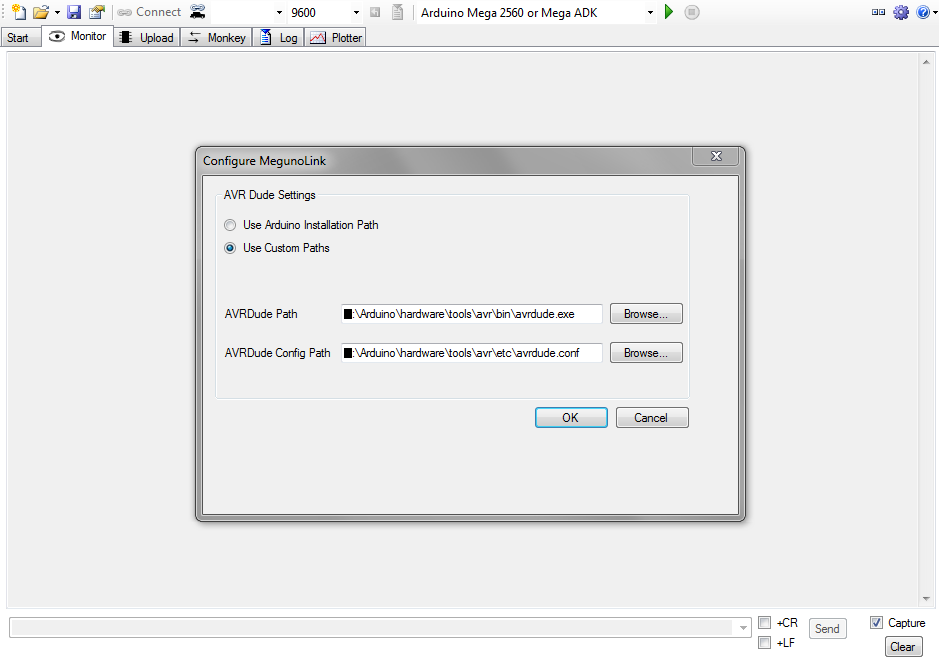
\includegraphics[width=0.85\textwidth]{Billeder/implementation/megunolink_config.png}
	\vspace{-.5cm}
	\caption{MegunoLink config}
	\label{fig:meglinkconf}
\end{figure}

For at kunne compilere, skal der linkes til projektets source fil. Hvis dette er udført korrekt, burde det være muligt at uploade source filen til arduino.

\subsection{Eksterne bibliotekter til Atmel}

Når dronen henter informationer ned fra serveren, sker det med en karakter af gangen. Dette giver nogle vanskeligheder ifht. at skulle sortere i dataet der er modtaget. Når der hentes data, kan det bl.a. være længde- og breddegrader. Når det modtages, ved man ikke hvilken plads det ligger på i arrayet og hvilken størrelse værdierne har. Man kan, mellem server og drone, forud definere størrelserne der sendes/modtages, men det er hverken dynamisk eller præcis. Fra server siden er flyveopsætningen defineret som JSon objekter, hvilket er overskueligt og nem at sortere i. \\
I Atmel eller arduino findes der ikke et standard JSon bibliotek, der kan søge eller erstatte informationerne i et JSon objekt. Derfor har det været nødvendigt at finde et bibliotek der har kunnet tage denne type fil og bearbejde det som almindeligt data. Det anvendte bibliotek hedder aJson\footnote{https://github.com/interactive-matter/aJson} og er et frit tilgængeligt JSon bibliotek.Dette bibliotek er kombatibel med arduino. Ved hjælp af dette bibliotek, er det blevet muligt at hente flyveopsætningen fra serveren og afkode, oprette og ændre i dataet.